\documentclass[conference]{IEEEtran}
\IEEEoverridecommandlockouts

\usepackage{cite}
\usepackage{amsmath,amssymb,amsfonts}
\usepackage{algorithmic}
\usepackage{graphicx}
\usepackage{textcomp}
\usepackage{xcolor}
\usepackage{listings}
\usepackage{float}
\usepackage[caption=false,font=footnotesize]{subfig}



\begin{document}

\title{Speech Enhancement System using Digital Signal Processing}

\author{
\IEEEauthorblockN{Muhsin M. Chowdhury}
\IEEEauthorblockA{
Electronics \& Instrumentation Engineering\\
School of Electrical Engineering\\
MIT Manipal\\
Karnataka, IN \\
muhsin.mitmpl2022@learner.manipal.edu
}
}

\maketitle

\begin{abstract}
Speech signals are often corrupted by noise during recording and transmission, which reduces their clarity and quality. This paper presents a simple speech enhancement system using digital signal processing techniques. The approach involves adding noise to a clean speech signal and then applying digital filters to reduce the noise. Finite Impulse Response (FIR) and Infinite Impulse Response (IIR) filters are designed and implemented in MATLAB for this purpose. The performance of the filters is evaluated by comparing the original, noisy, and filtered signals using graphical analysis. The results demonstrate that both FIR and IIR filters effectively improve the quality of the speech signal, with each method having its own advantages.
\end{abstract}

\begin{IEEEkeywords}
Speech Enhancement, Digital Signal Processing, FIR Filter, IIR Filter, MATLAB
\end{IEEEkeywords}

\section{Introduction}

Speech is one of the most common ways in which people communicate. In practical situations, speech signals are often affected by unwanted noise during recording or transmission. This noise reduces clarity and makes the signal difficult to understand.

Speech enhancement is the process of improving the quality of a speech signal by reducing noise. It is widely used in applications such as mobile communication, hearing aids, and voice-controlled systems. Various techniques are available for speech enhancement, but many of them are complex and require high computational resources.

In this work, a simple approach is followed using digital signal processing techniques. The focus is on using Finite Impulse Response (FIR) and Infinite Impulse Response (IIR) filters to reduce noise from a speech signal. A clean speech signal is first taken and noise is added to it. Then, FIR and IIR filters are applied to improve the signal quality.

The entire system is implemented in MATLAB. The performance of the filters is studied by comparing the original, noisy, and filtered signals using graphical analysis. This approach helps in understanding the basic concepts of speech enhancement in a simple and practical way.

\section{Problem Statement}

In real-world environments, speech signals are often affected by noise during recording or transmission. This noise makes the speech signal unclear and reduces its intelligibility.

The problem addressed in this work is to recover a cleaner version of the speech signal from a noisy input. The noisy signal can be considered as a combination of the original speech signal and unwanted noise.

The objective of this work is to design and implement simple digital filtering techniques to reduce noise from speech signals. In particular, FIR and IIR filters are used and their performance is compared based on both visual and quantitative analysis.

\section{Literature Survey}

Several methods have been developed for improving the quality of speech signals affected by noise. One of the basic approaches involves the use of digital filters such as Finite Impulse Response (FIR) and Infinite Impulse Response (IIR) filters. These filters are widely used due to their simplicity and ease of implementation.

FIR filters are known for their stability and linear phase characteristics, which help in preserving the shape of the signal. IIR filters, on the other hand, are more efficient and require fewer coefficients to achieve similar performance.

More advanced techniques such as spectral subtraction and adaptive filtering are also used for speech enhancement. However, these methods are more complex and require higher computational effort.

In this work, simple FIR and IIR filtering techniques are used to enhance speech signals, as they are suitable for basic understanding and practical implementation.

\section{Methodology}

The proposed speech enhancement system follows a simple and structured approach using digital filters. The overall process starts with a clean speech signal, which is then affected by noise. The noisy signal is processed using FIR and IIR filters to reduce the noise and improve clarity.

The main steps involved in the system are as follows:

\begin{enumerate}
    \item Load a clean speech signal in MATLAB.
    \item Add noise to the speech signal to simulate real-world conditions.
    \item Design an FIR filter using standard filter design functions.
    \item Design an IIR filter using the Butterworth method.
    \item Apply both filters to the noisy signal.
    \item Compare the original, noisy, and filtered signals.
\end{enumerate}

The FIR filter is based on a non-recursive structure and uses only present and past input values. The general form of the FIR filter is given by:

\begin{equation}
y[n] = \sum_{k=0}^{N} b_k x[n-k]
\end{equation}

The IIR filter uses a recursive structure, where past output values are also used along with input values. This makes the filter more efficient but slightly complex.

A block diagram of the proposed system is shown in Fig.~\ref{fig:block_diagram}.

\begin{figure}[htbp]
\centering
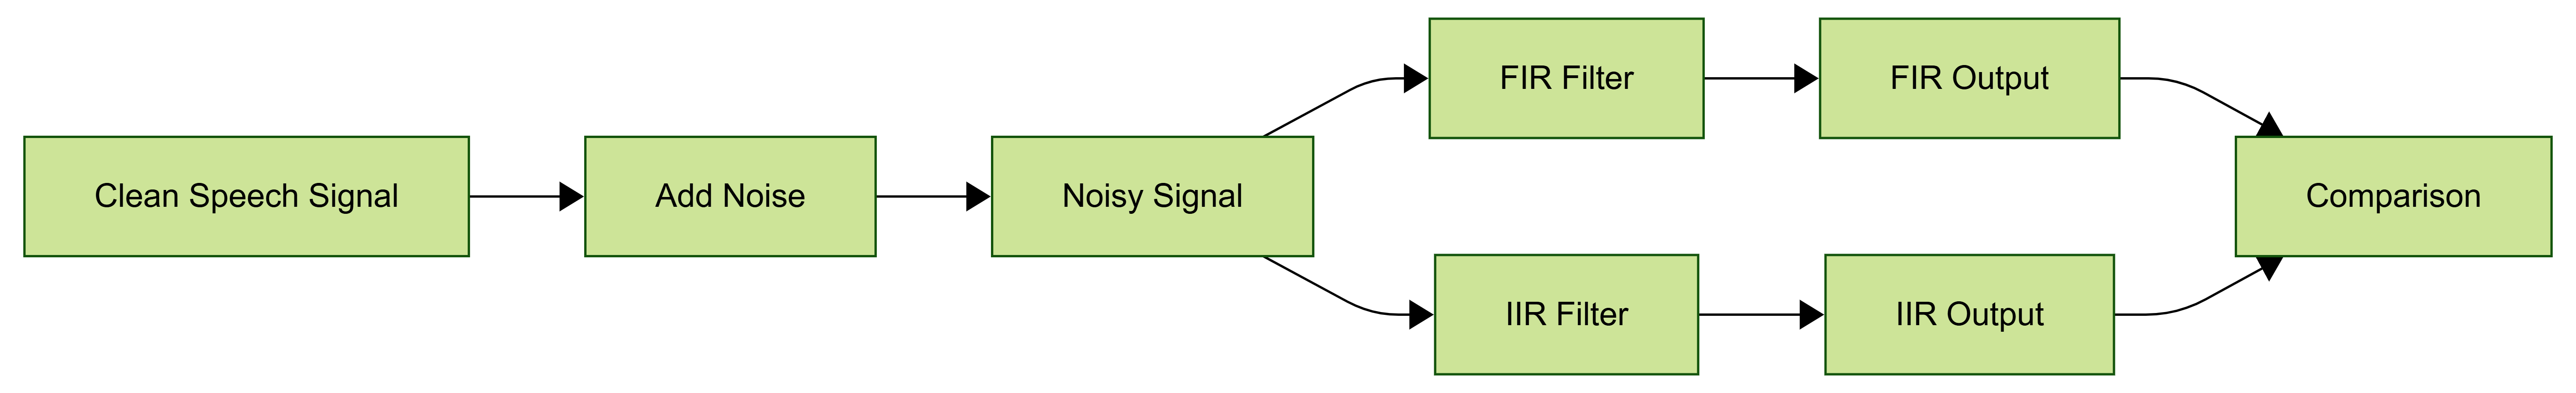
\includegraphics[width=0.9\columnwidth,height=4.2cm,keepaspectratio]{block_diagram.png}
\caption{Block diagram of the speech enhancement system}
\label{fig:block_diagram}
\end{figure}

\section{Implementation}

The proposed speech enhancement system is implemented using MATLAB. The process involves loading a speech signal from an audio file, adding synthetic white Gaussian noise, designing FIR and IIR low-pass filters, and applying them to improve the signal quality. The current implementation also saves time-domain plots, frequency-domain plots, and filter responses for documentation.

\subsection{Loading the Speech Signal}

A speech signal in \texttt{.wav} format is loaded into MATLAB using the \texttt{audioread} function. If the file contains stereo audio, only the left channel is used so that the subsequent processing is performed on a single speech waveform.

\begin{lstlisting}[basicstyle=\footnotesize\ttfamily, breaklines=true]
[x, fs] = audioread('audio.wav');
x = x(:,1)';
t = (0:length(x)-1) / fs;
\end{lstlisting}

\subsection{Adding Noise}

Noise is added to the clean speech signal to simulate real-world conditions.

\begin{lstlisting}[basicstyle=\footnotesize\ttfamily, breaklines=true]
noise_power = 0.05;
noisy_signal = x + noise_power * randn(size(x));
\end{lstlisting}

\subsection{Design of FIR Filter}

An FIR low-pass filter is designed using the \texttt{fir1} function with order 50 and cutoff frequency 3400~Hz, normalized by the Nyquist frequency.

\begin{lstlisting}[basicstyle=\footnotesize\ttfamily, breaklines=true]
fir_order = 50;
fir_cutoff = 3400 / (fs/2);
b_fir = fir1(fir_order, fir_cutoff);
fir_output = filter(b_fir, 1, noisy_signal);
\end{lstlisting}


\subsection{Design of IIR Filter}

An IIR Butterworth low-pass filter is designed using the \texttt{butter} function with order 4 and the same 3400~Hz cutoff frequency.

\begin{lstlisting}[basicstyle=\footnotesize\ttfamily, breaklines=true]
iir_order = 4;
iir_cutoff = 3400 / (fs/2);
[b_iir, a_iir]=butter(iir_order,iir_cutoff,'low');
iir_output = filter(b_iir, a_iir, noisy_signal);
\end{lstlisting}

\subsection{Plotting the Signals}

The original, noisy, and filtered signals are plotted separately for comparison, and each figure is exported for inclusion in the report.

\begin{lstlisting}[basicstyle=\footnotesize\ttfamily, breaklines=true]
figure; plot(t, x);
title('Original Speech Signal');
saveas(gcf, 'original_signal.png');

figure; plot(t, noisy_signal);
title('Noisy Speech Signal');
saveas(gcf, 'noisy_signal.png');
\end{lstlisting}

\section{Results}

The performance of the speech enhancement system is evaluated by comparing the original, noisy, and filtered speech signals. The comparison is carried out using time-domain plots, while additional FFT plots and filter responses are generated during execution for further analysis.


\subsection{Original and Noisy Signals}

The original speech signal is shown in Fig.~\ref{fig:original}. The waveform is smooth and represents clean speech. After adding noise, the signal becomes irregular as shown in Fig.~\ref{fig:noisy}. The fluctuations in amplitude indicate the presence of noise.

\begin{figure}[htbp]
\centering
\subfloat[Original speech signal\label{fig:original}]{
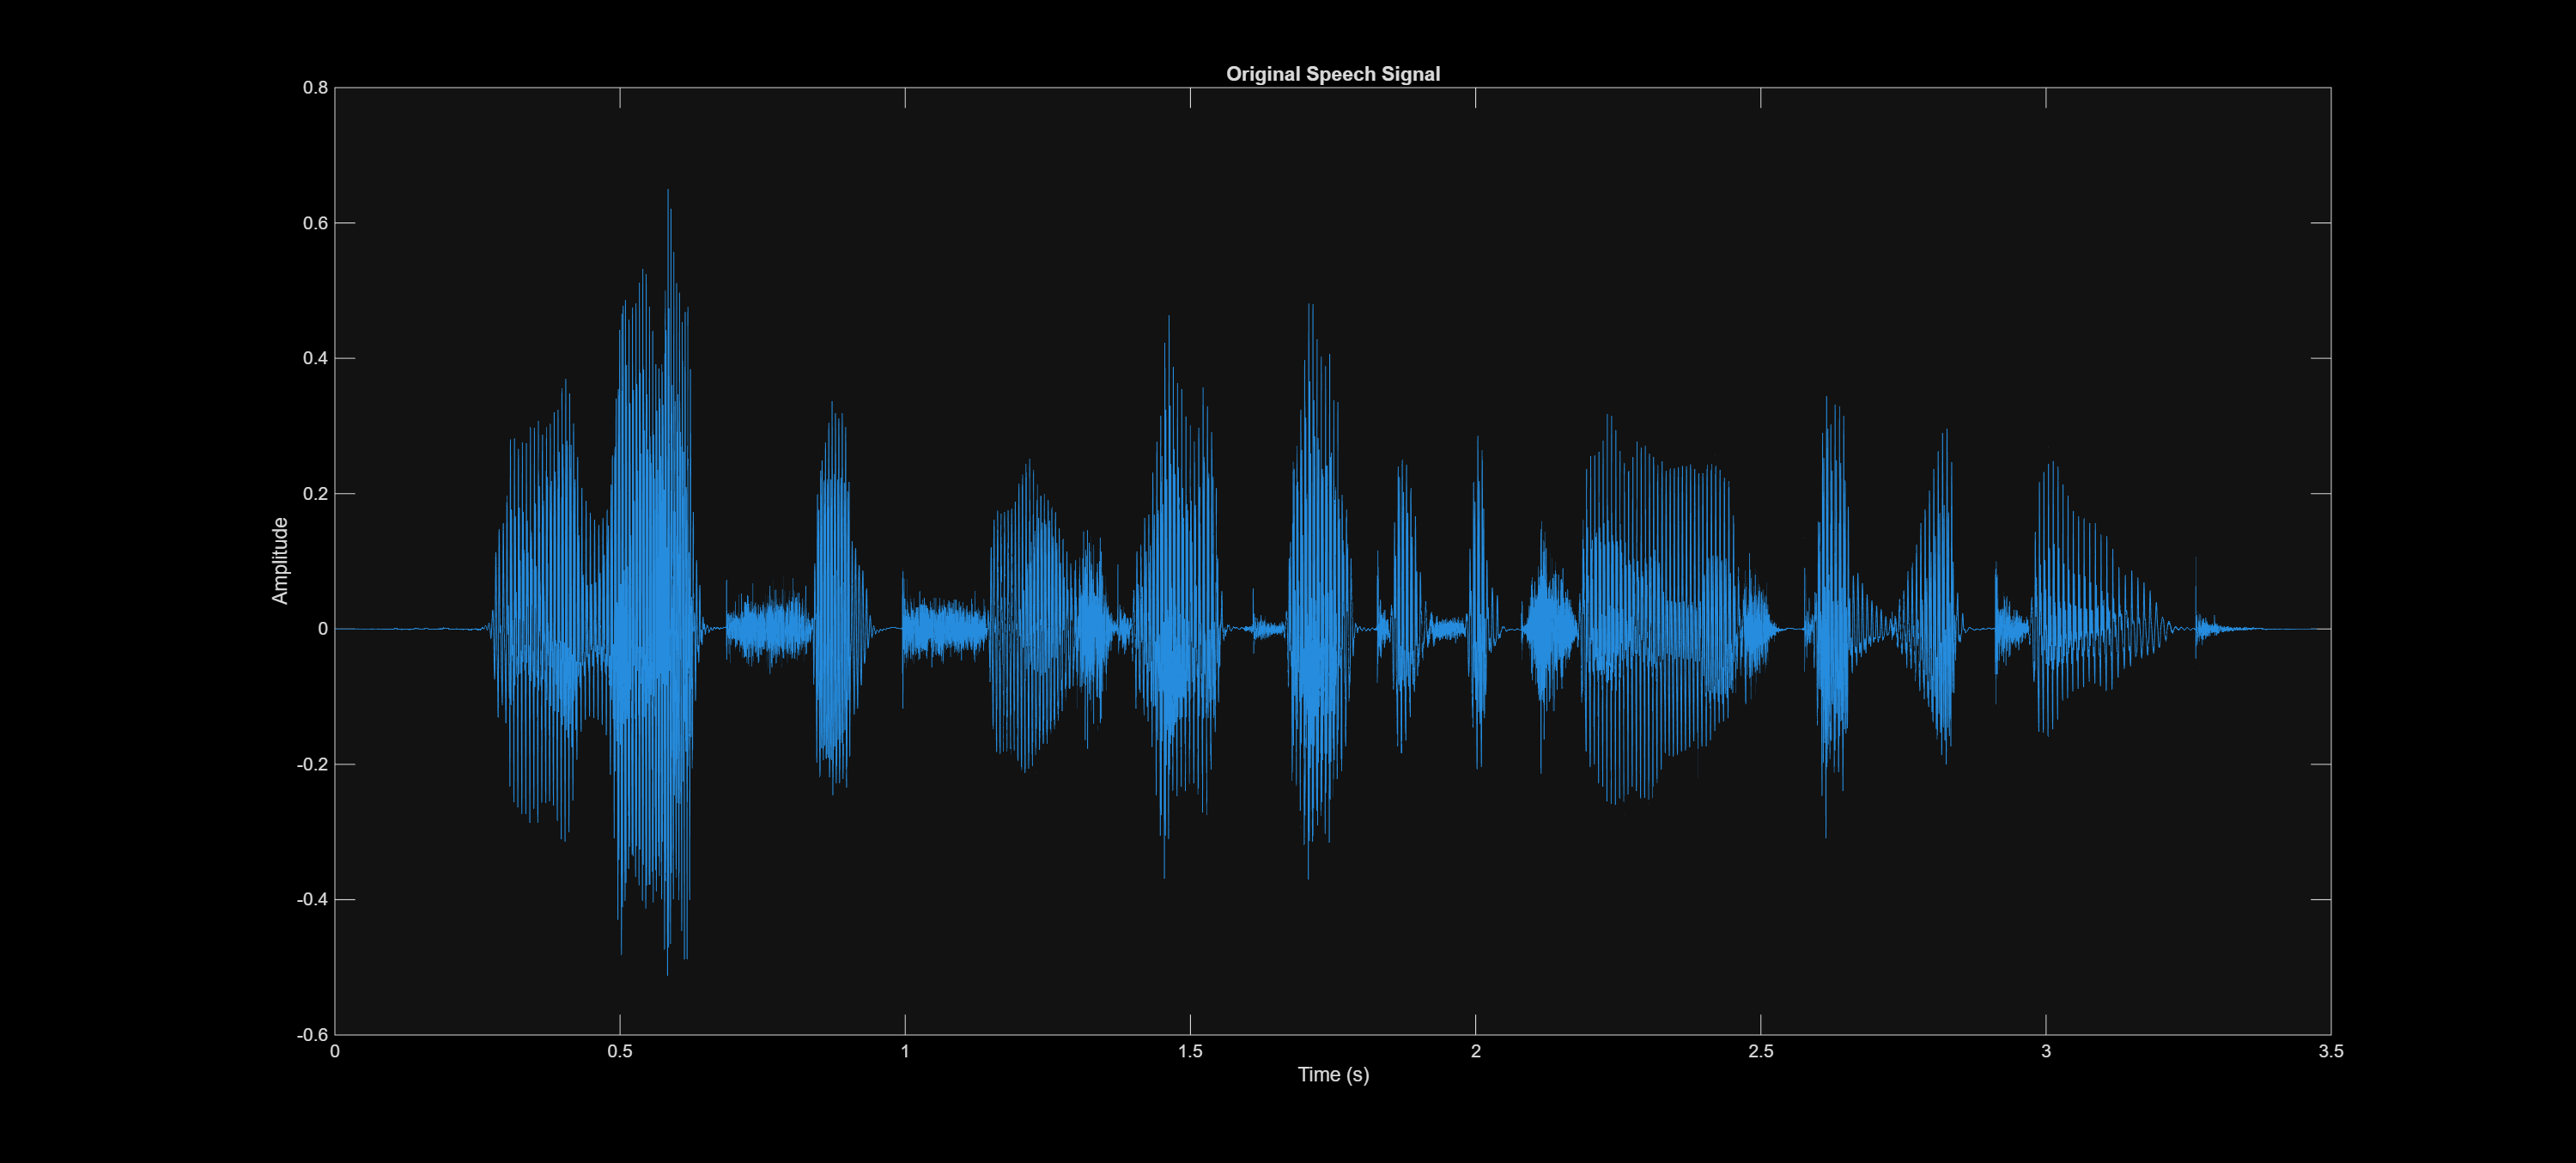
\includegraphics[width=0.48\columnwidth,height=3.5cm,keepaspectratio]{original_signal.png}
}
\hfill
\subfloat[Noisy speech signal\label{fig:noisy}]{
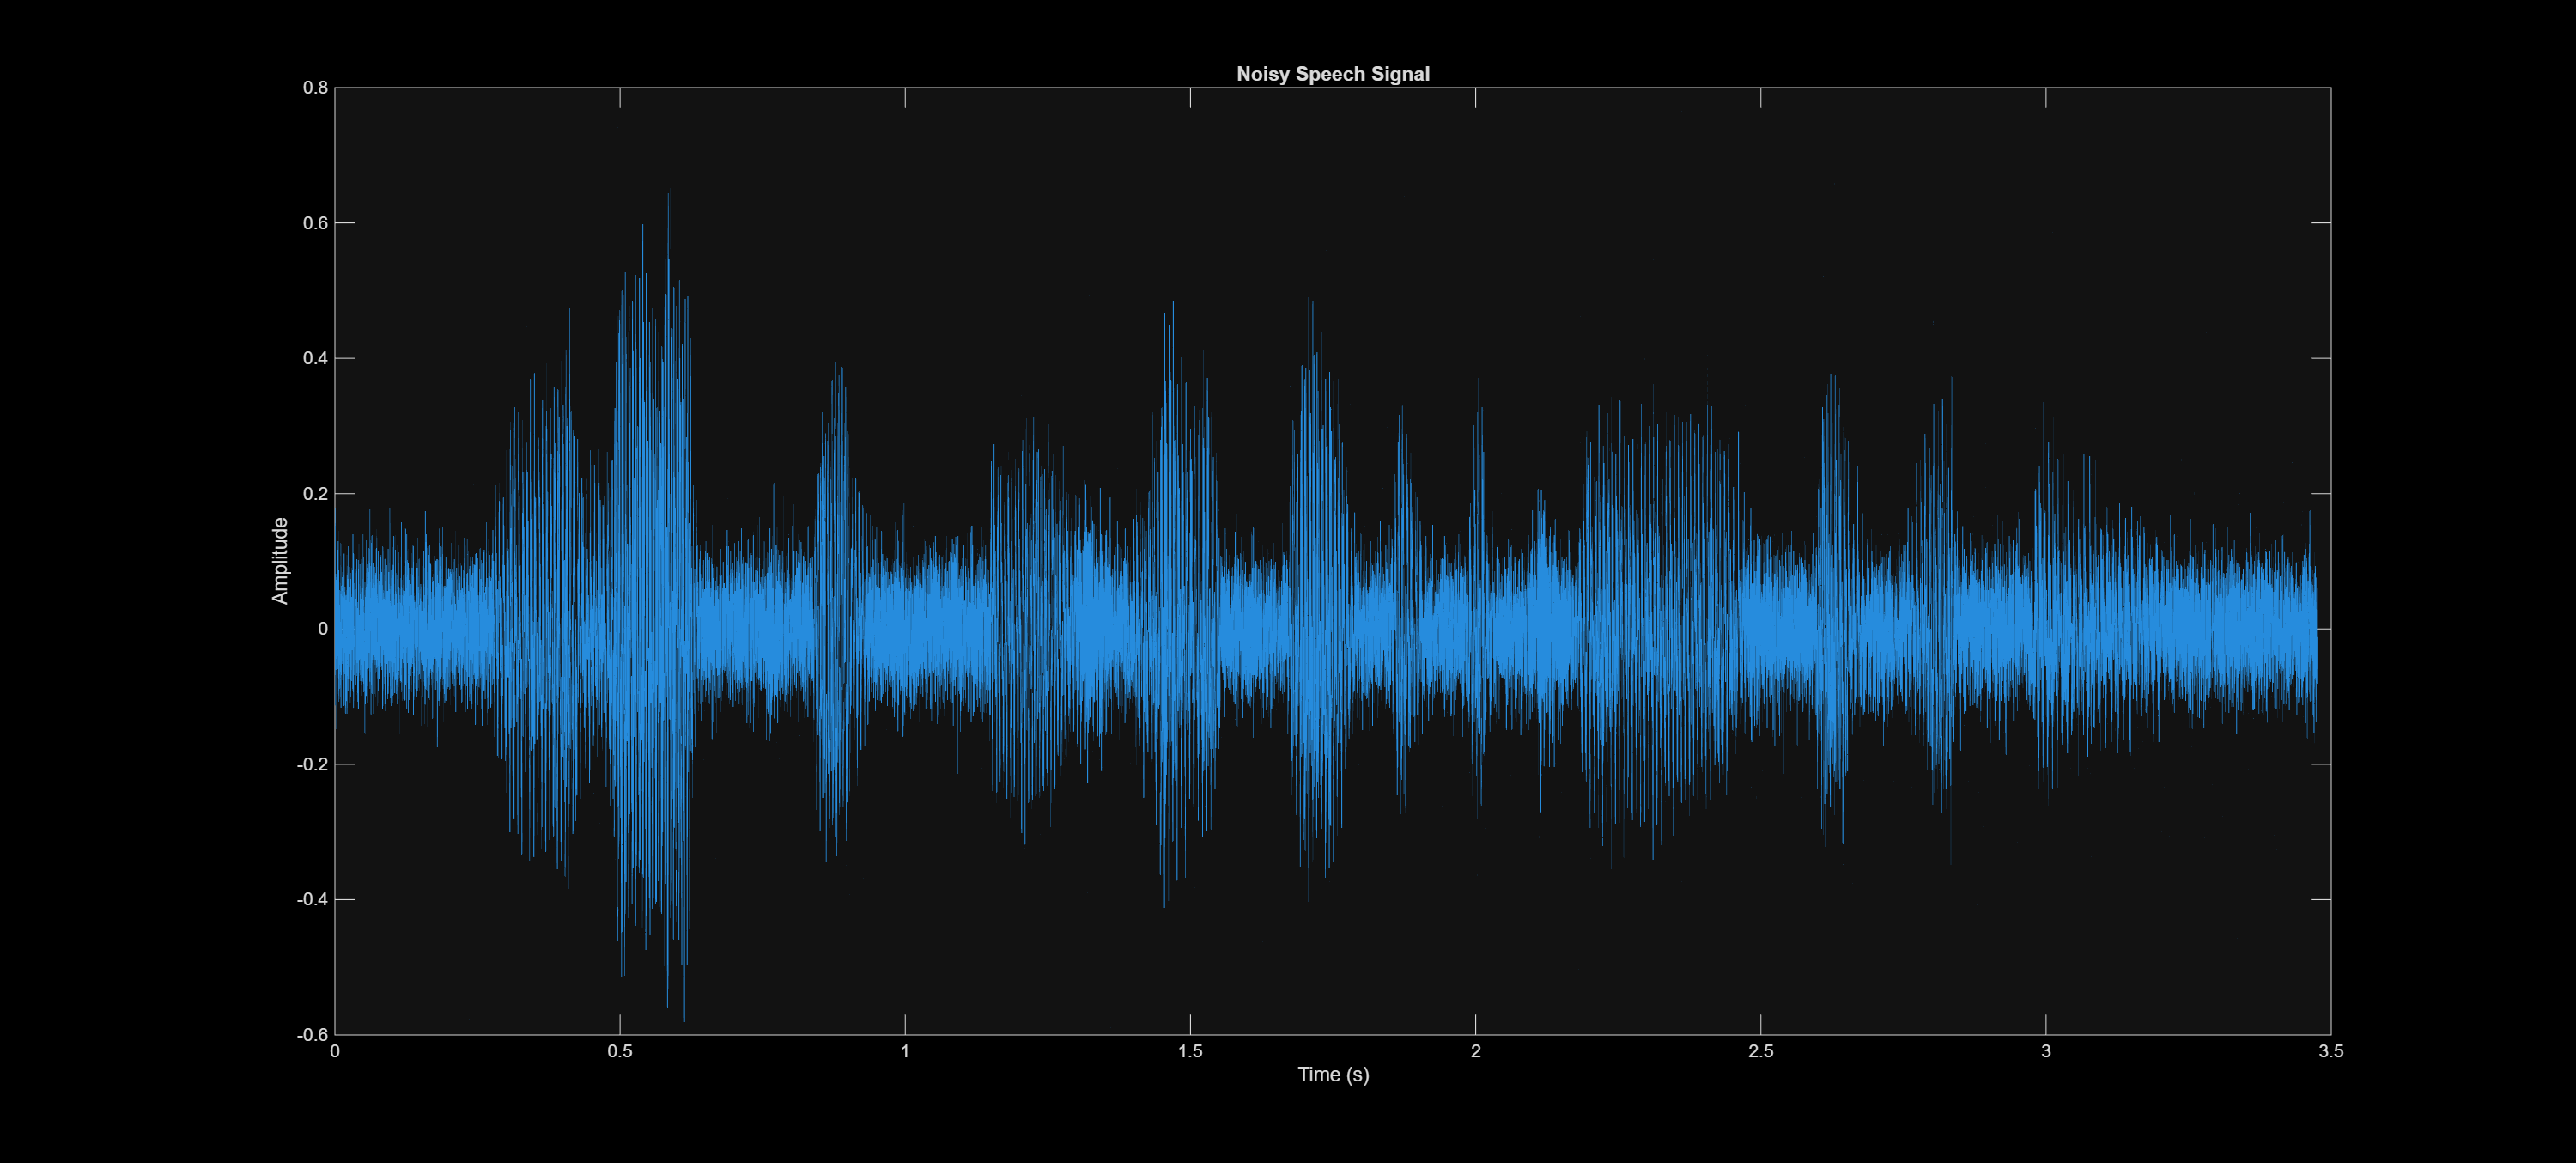
\includegraphics[width=0.48\columnwidth,height=3.5cm,keepaspectratio]{noisy_signal.png}
}
\caption{Comparison of the original and noisy speech waveforms}
\end{figure}

\subsection{Filtered Signals}

The output of the FIR filter is shown in Fig.~\ref{fig:fir}. The noise level is reduced and the signal appears smoother compared to the noisy signal.

The output of the IIR filter is shown in Fig.~\ref{fig:iir}. The signal becomes clearer and the noise is reduced effectively with fewer computations.

\begin{figure}[htbp]
\centering
\subfloat[FIR filter output\label{fig:fir}]{
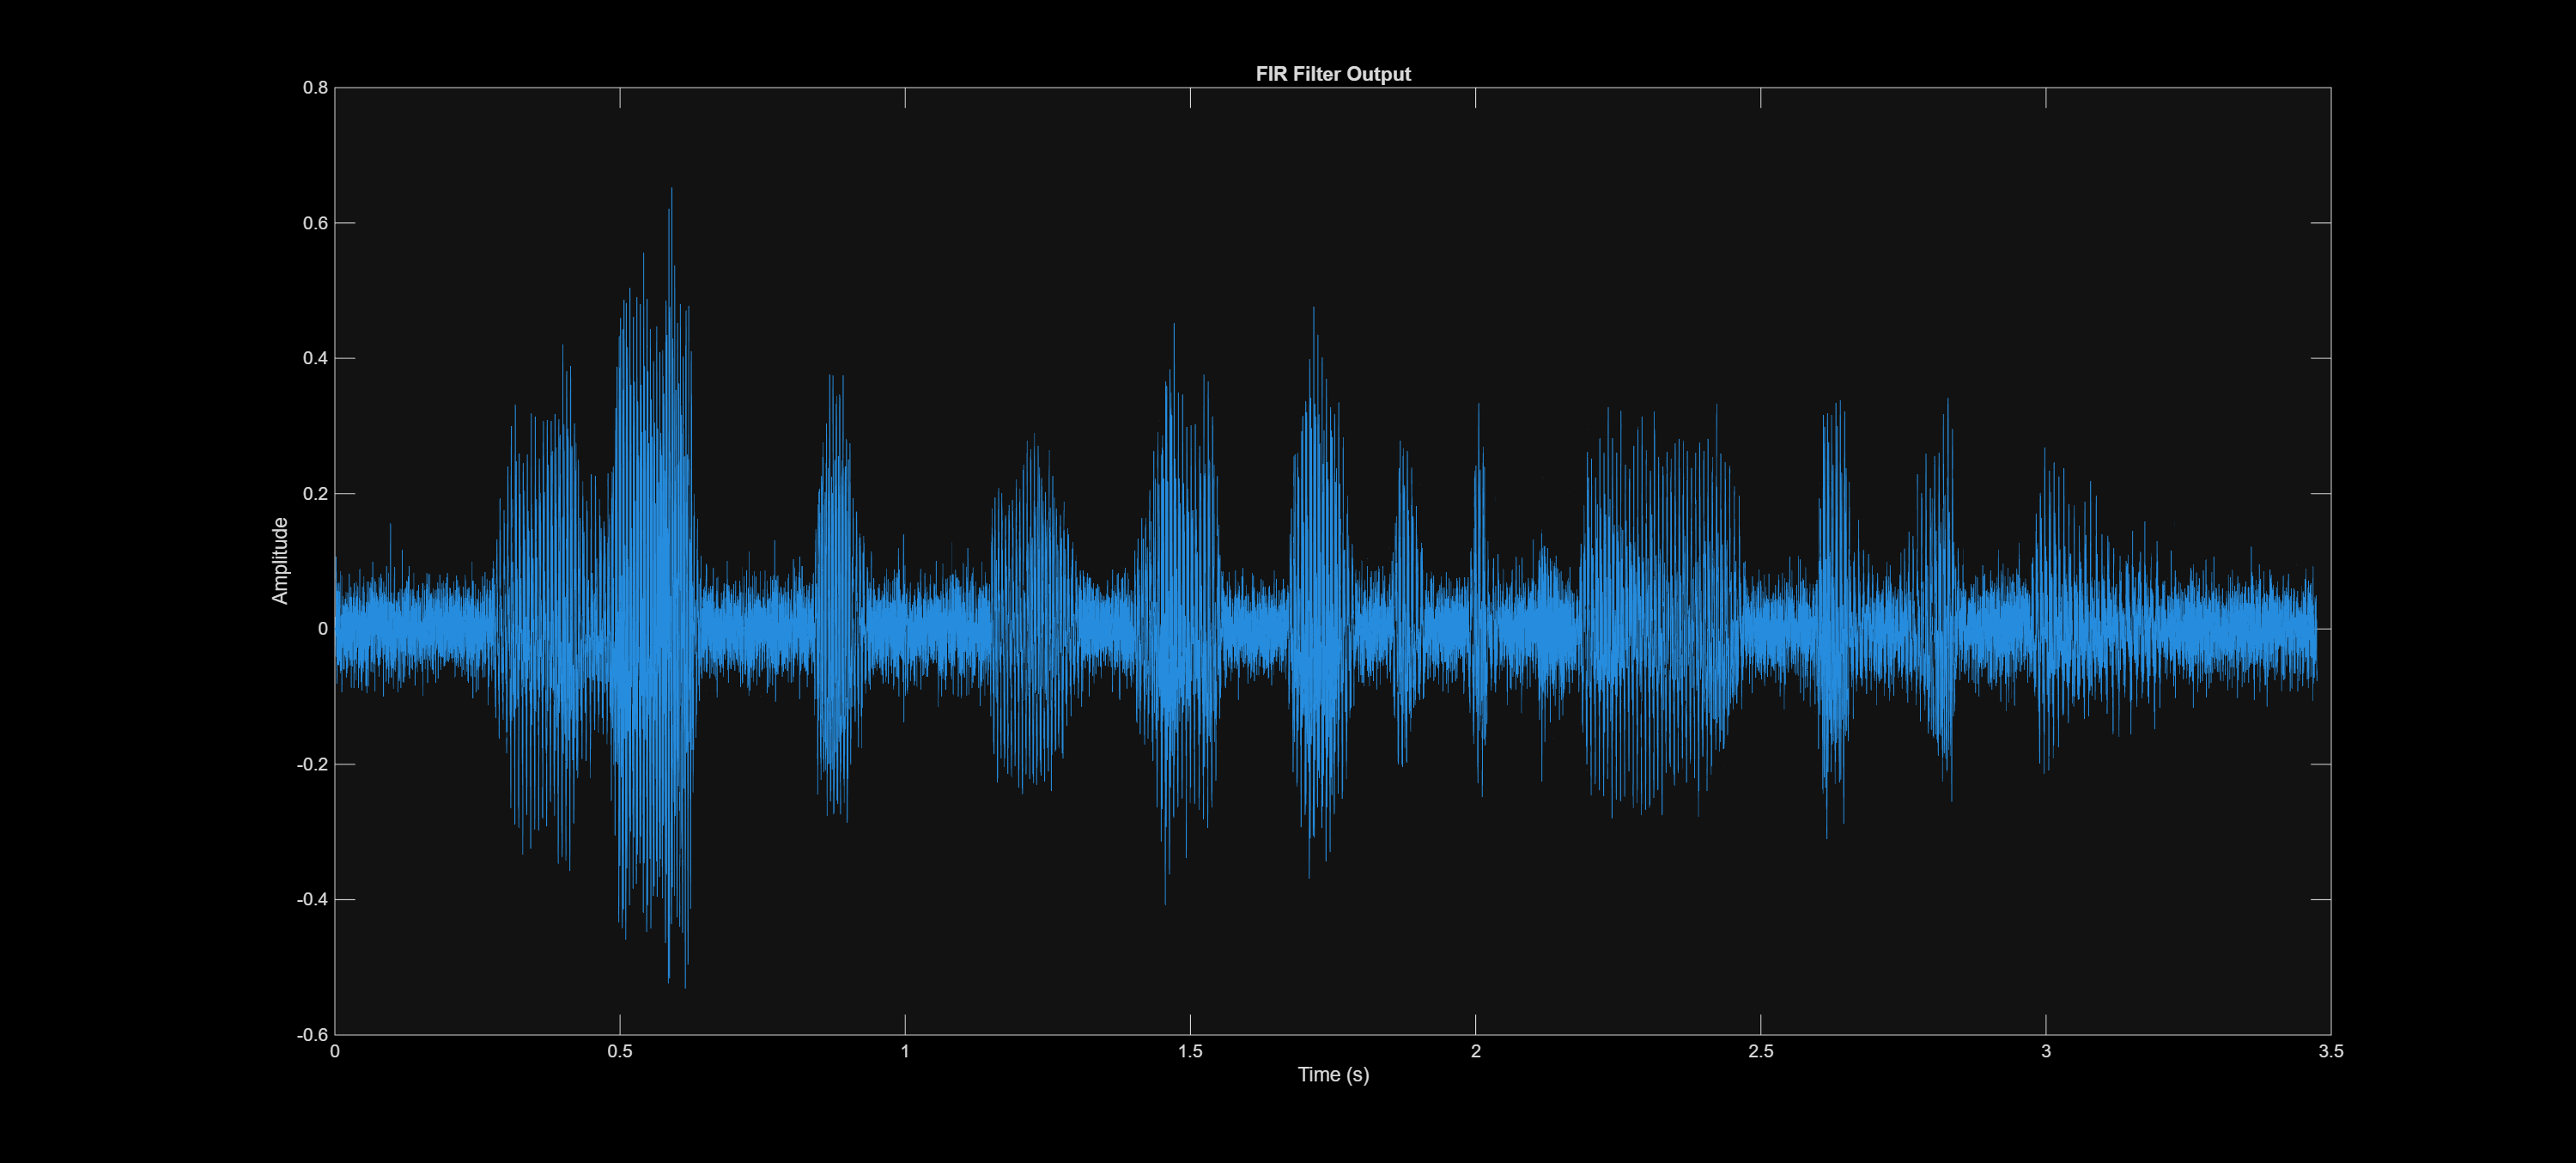
\includegraphics[width=0.48\columnwidth,height=3.5cm,keepaspectratio]{fir_output.png}
}
\hfill
\subfloat[IIR filter output\label{fig:iir}]{
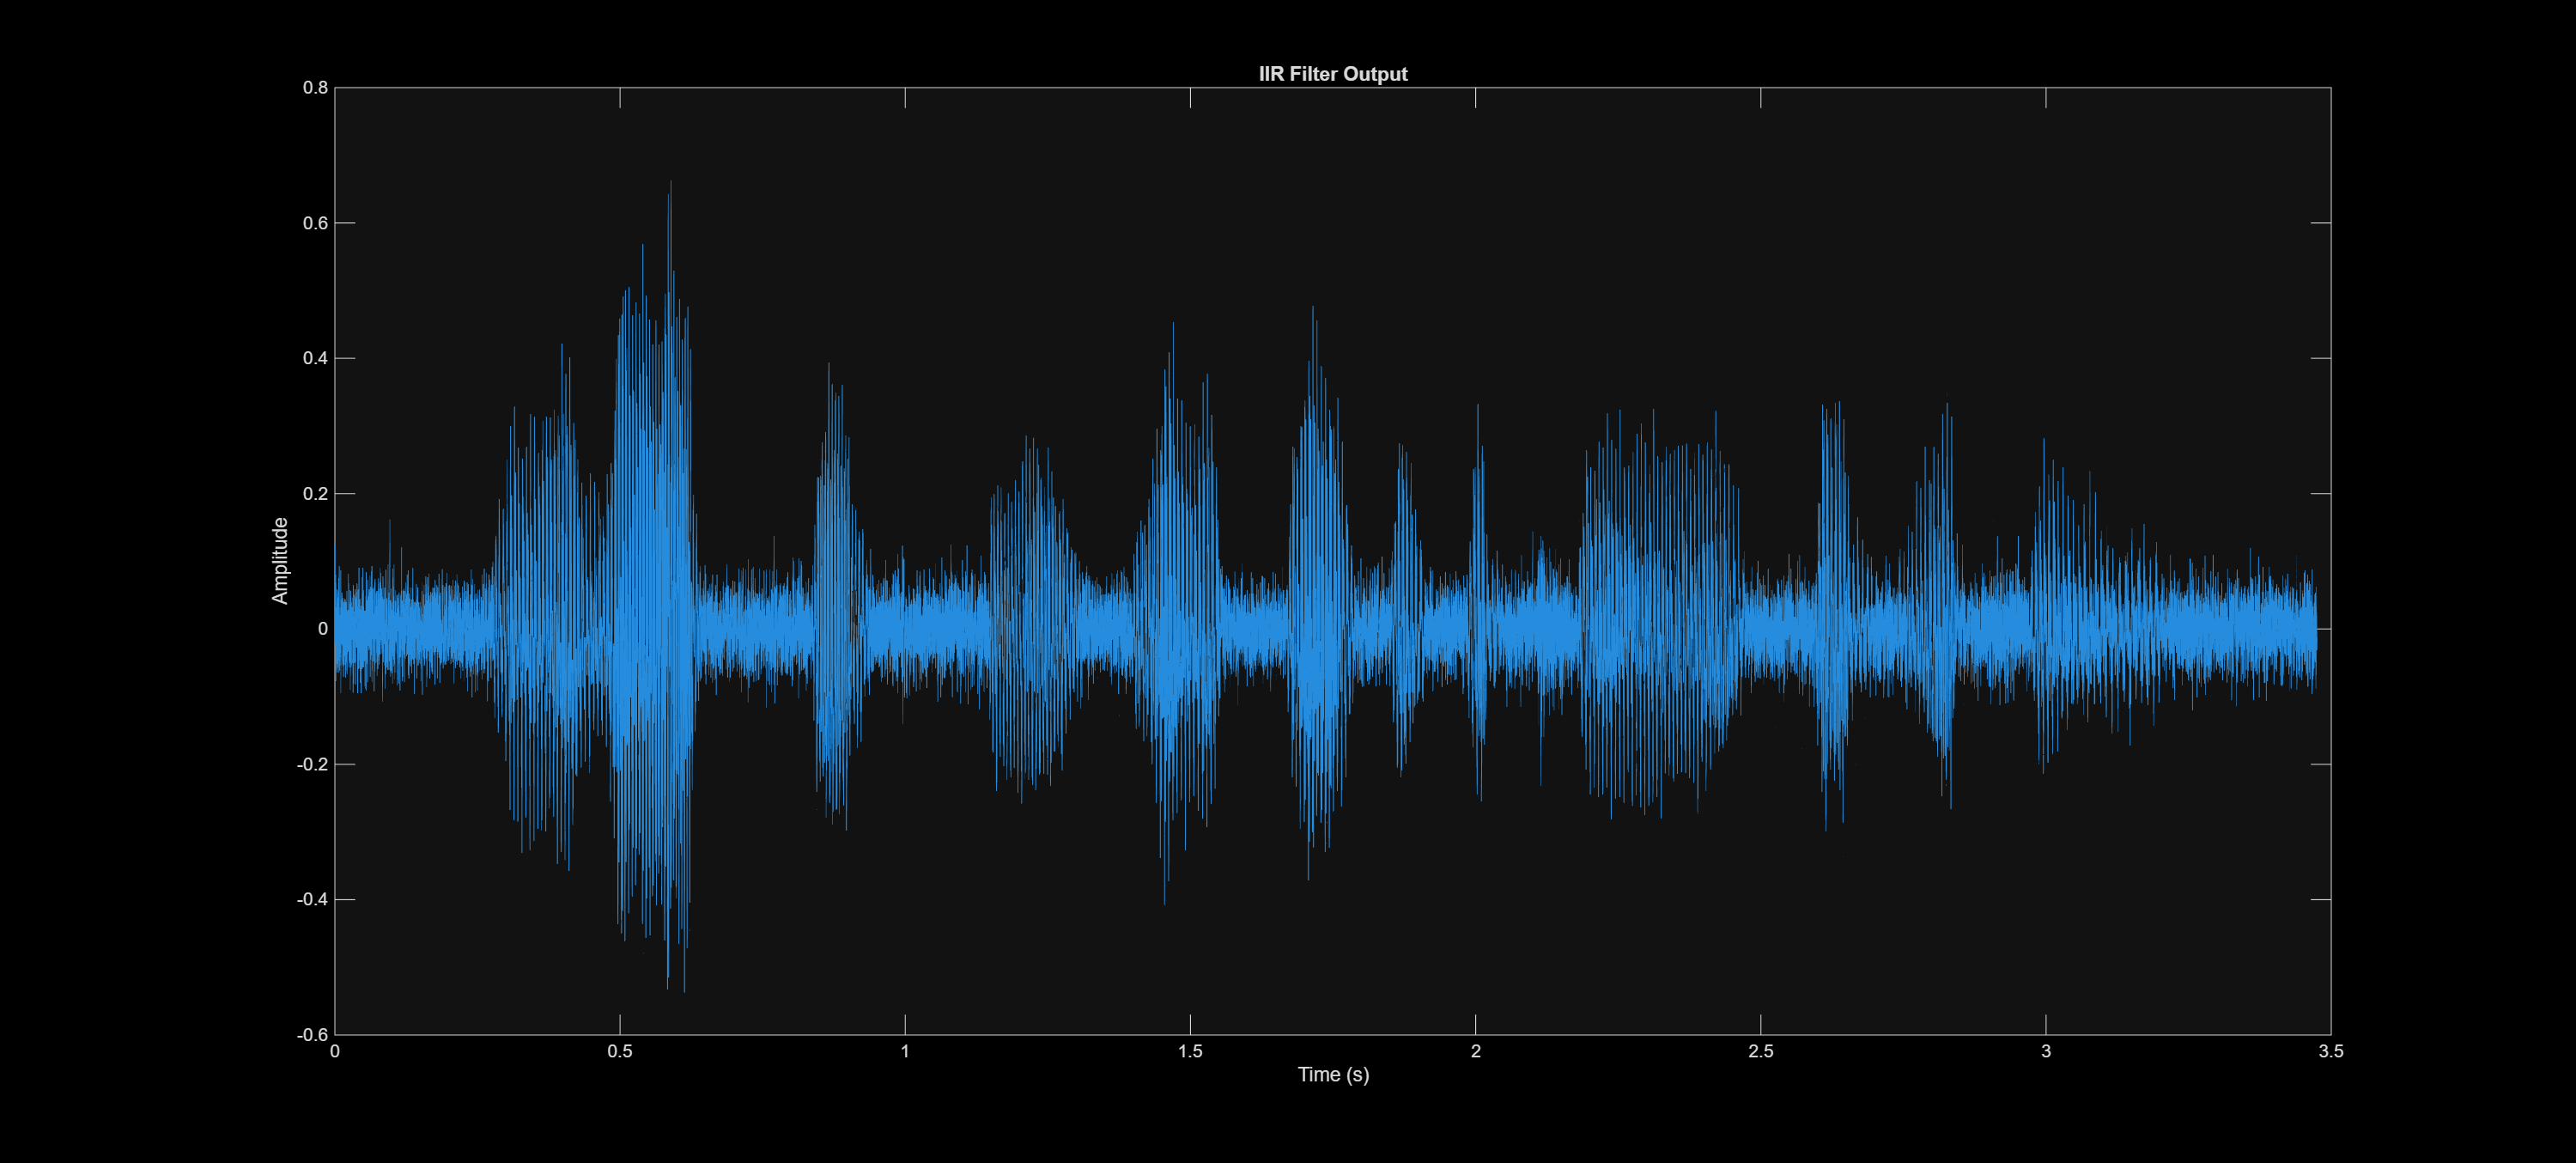
\includegraphics[width=0.48\columnwidth,height=3.5cm,keepaspectratio]{iir_output.png}
}
\caption{Comparison of the FIR and IIR filtered speech waveforms}
\end{figure}

From the results, it can be observed that both filters improve the quality of the speech signal. The filtered signals are closer to the original signal compared to the noisy signal. The MATLAB implementation also computes Signal-to-Noise Ratio (SNR) and Mean Squared Error (MSE) values for the noisy, FIR-filtered, and IIR-filtered signals, which provide a quantitative basis for comparison in addition to visual inspection.

\subsection{Quantitative Performance Evaluation}

In addition to visual analysis, quantitative metrics are used to evaluate the performance of the speech enhancement system. Signal-to-Noise Ratio (SNR) and Mean Square Error (MSE) are calculated for the noisy and filtered signals.

SNR measures the strength of the signal relative to noise, while MSE measures the average squared difference between the original and processed signals.

\begin{table}[htbp]
\centering
\caption{Performance Comparison of Noisy, FIR, and IIR Signals}
\begin{tabular}{|c|c|c|c|}
\hline
Metric & Noisy Signal & FIR Output & IIR Output \\
\hline
SNR (dB) & 4.77 & -3.68 & 5.64 \\
MSE & 0.002494 & 0.017465 & 0.002041 \\
\hline
\end{tabular}
\end{table}

From the results, it can be observed that the IIR filter improves the SNR and reduces the MSE compared to the noisy signal, indicating effective noise reduction.

However, the FIR filter shows a decrease in SNR and an increase in MSE, which indicates that the chosen filter parameters are not optimal for the given signal. This suggests that improper selection of filter order or cutoff frequency can degrade the signal quality instead of improving it.

This analysis highlights the importance of proper filter design in speech enhancement systems.

Further improvement in FIR performance can be achieved by tuning the filter order and cutoff frequency.

\subsection{Frequency Domain Analysis}

While the time-domain plots provide a visual understanding of the signal behavior, further insight can be obtained by examining the signals in the frequency domain. This helps in understanding how noise is distributed across different frequencies and how effectively it is removed by the filters.

The frequency spectrum of the original signal shows the dominant frequency components of speech. After adding noise, the spectrum of the noisy signal becomes more spread out, indicating the presence of unwanted high-frequency components.

\begin{figure}[htbp]
\centering
\subfloat[Frequency spectrum of original speech signal]{
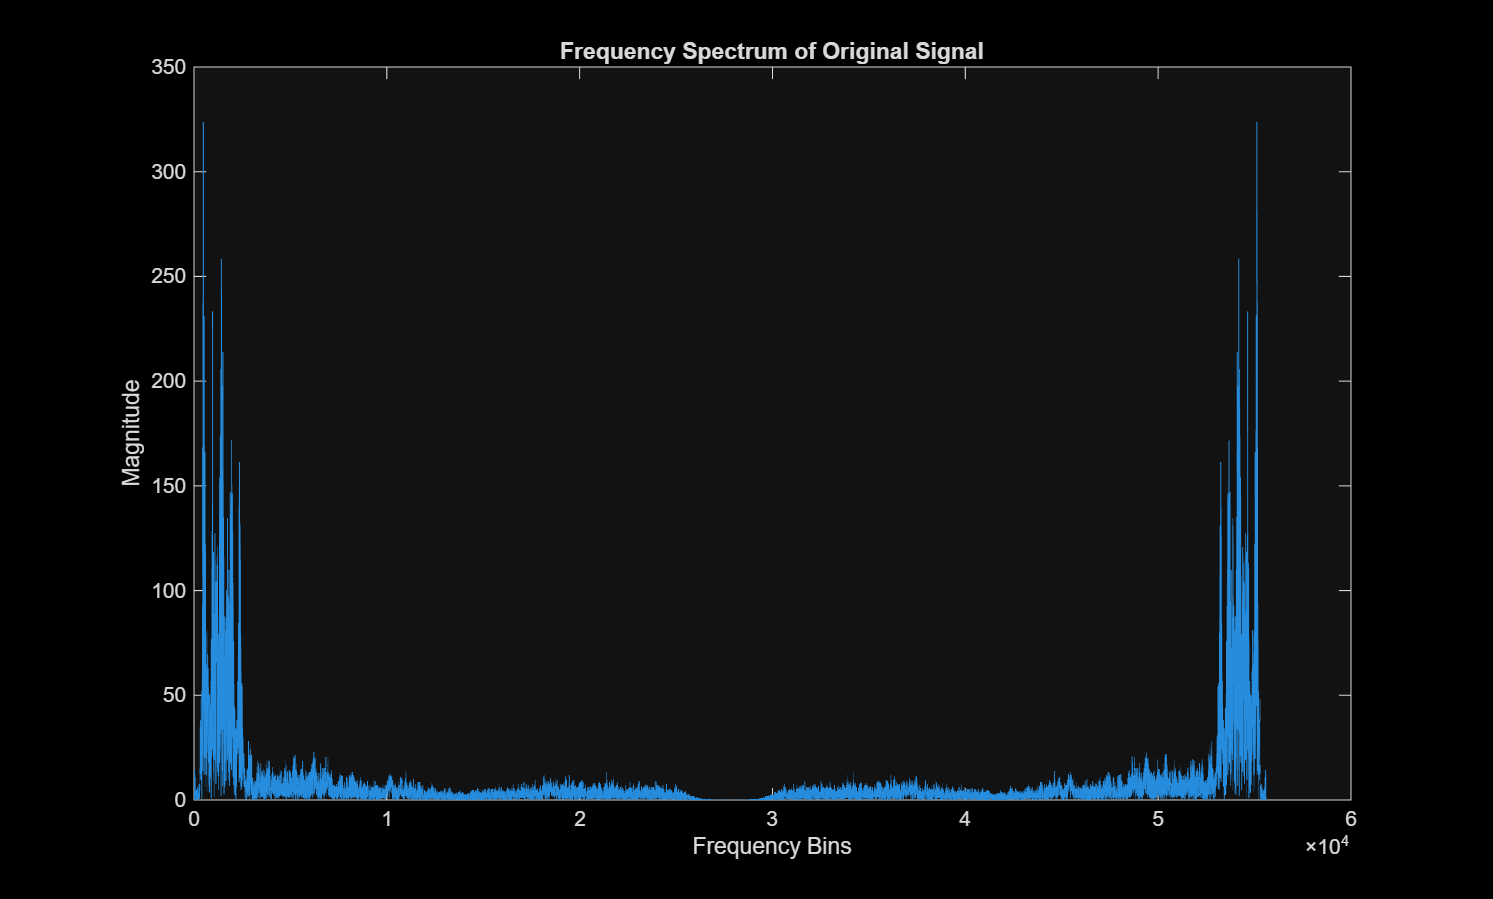
\includegraphics[width=0.48\columnwidth,height=3.3cm,keepaspectratio]{fft_original.png}
}
\hfill
\subfloat[Frequency spectrum of noisy speech signal]{
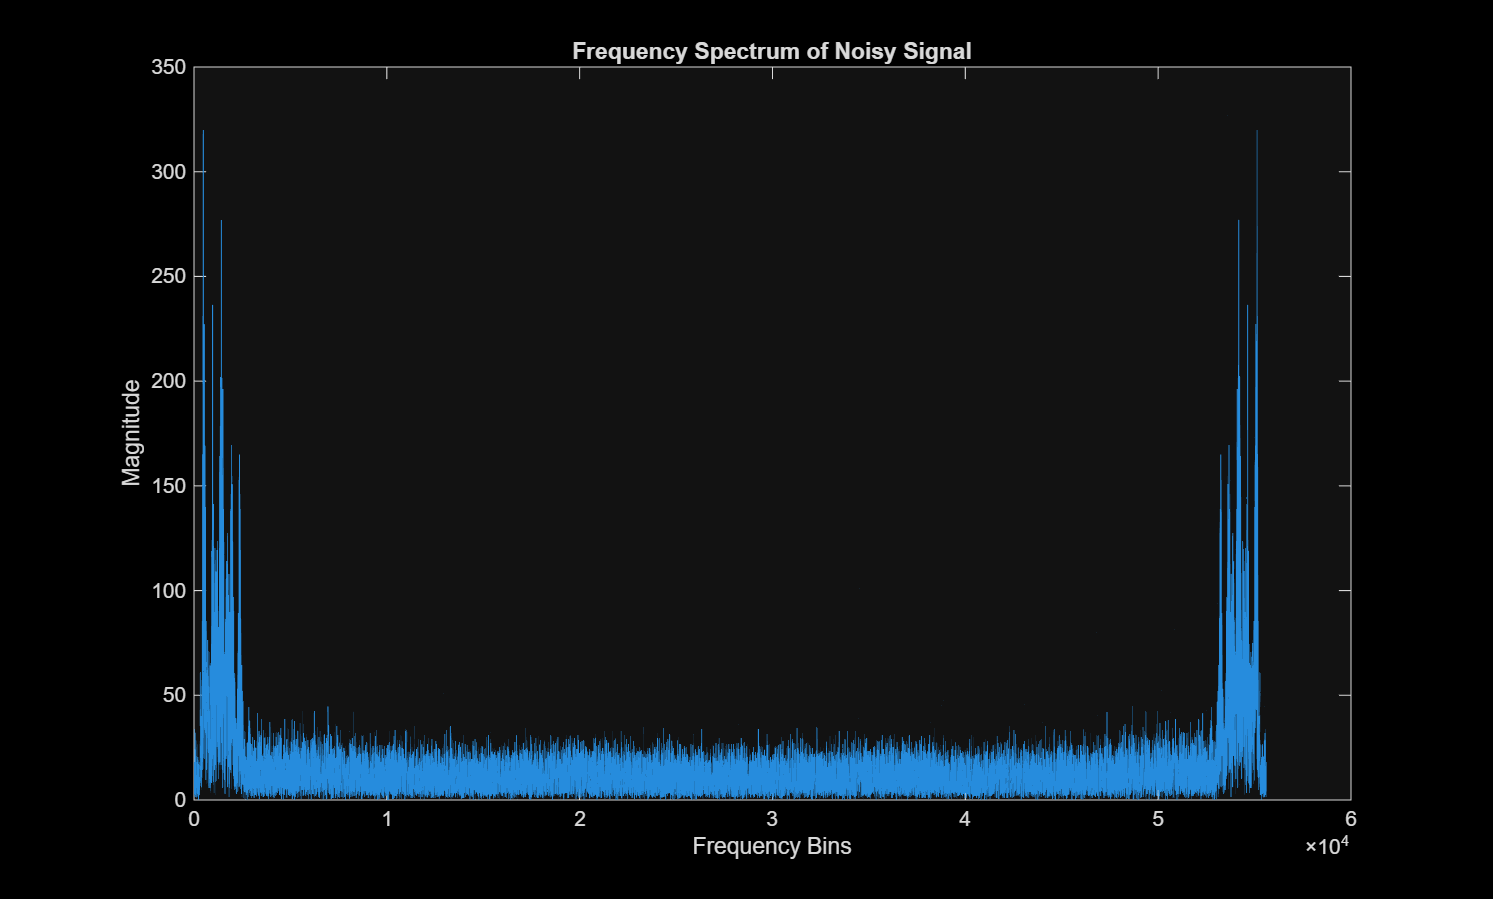
\includegraphics[width=0.48\columnwidth,height=3.3cm,keepaspectratio]{fft_noisy.png}
}

\vspace{2mm}

\subfloat[Frequency spectrum after FIR filtering]{
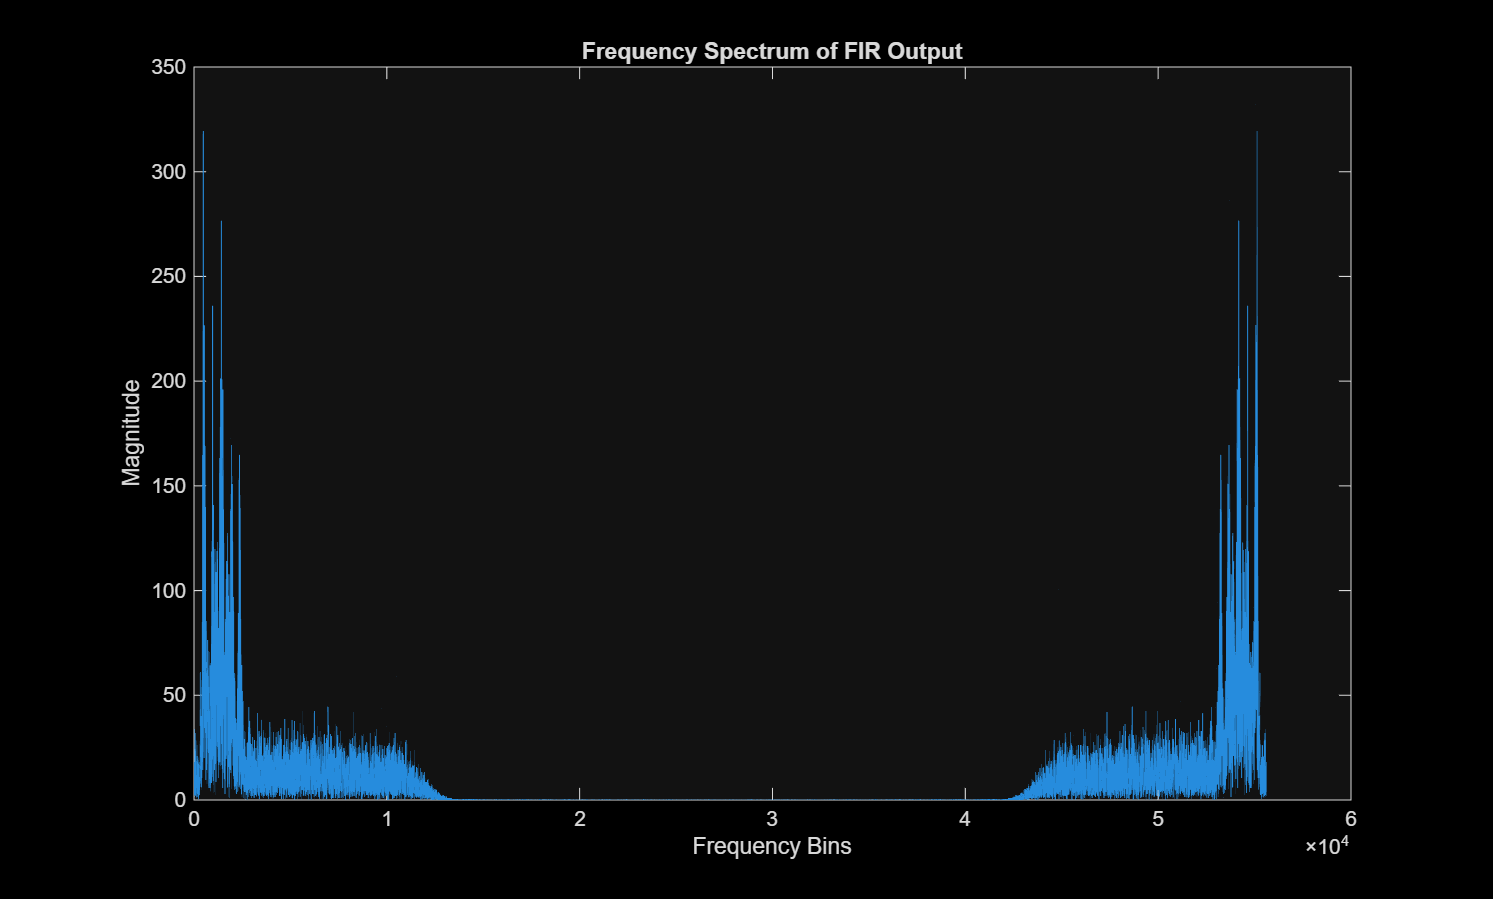
\includegraphics[width=0.48\columnwidth,height=3.3cm,keepaspectratio]{fft_fir.png}
}
\hfill
\subfloat[Frequency spectrum after IIR filtering]{
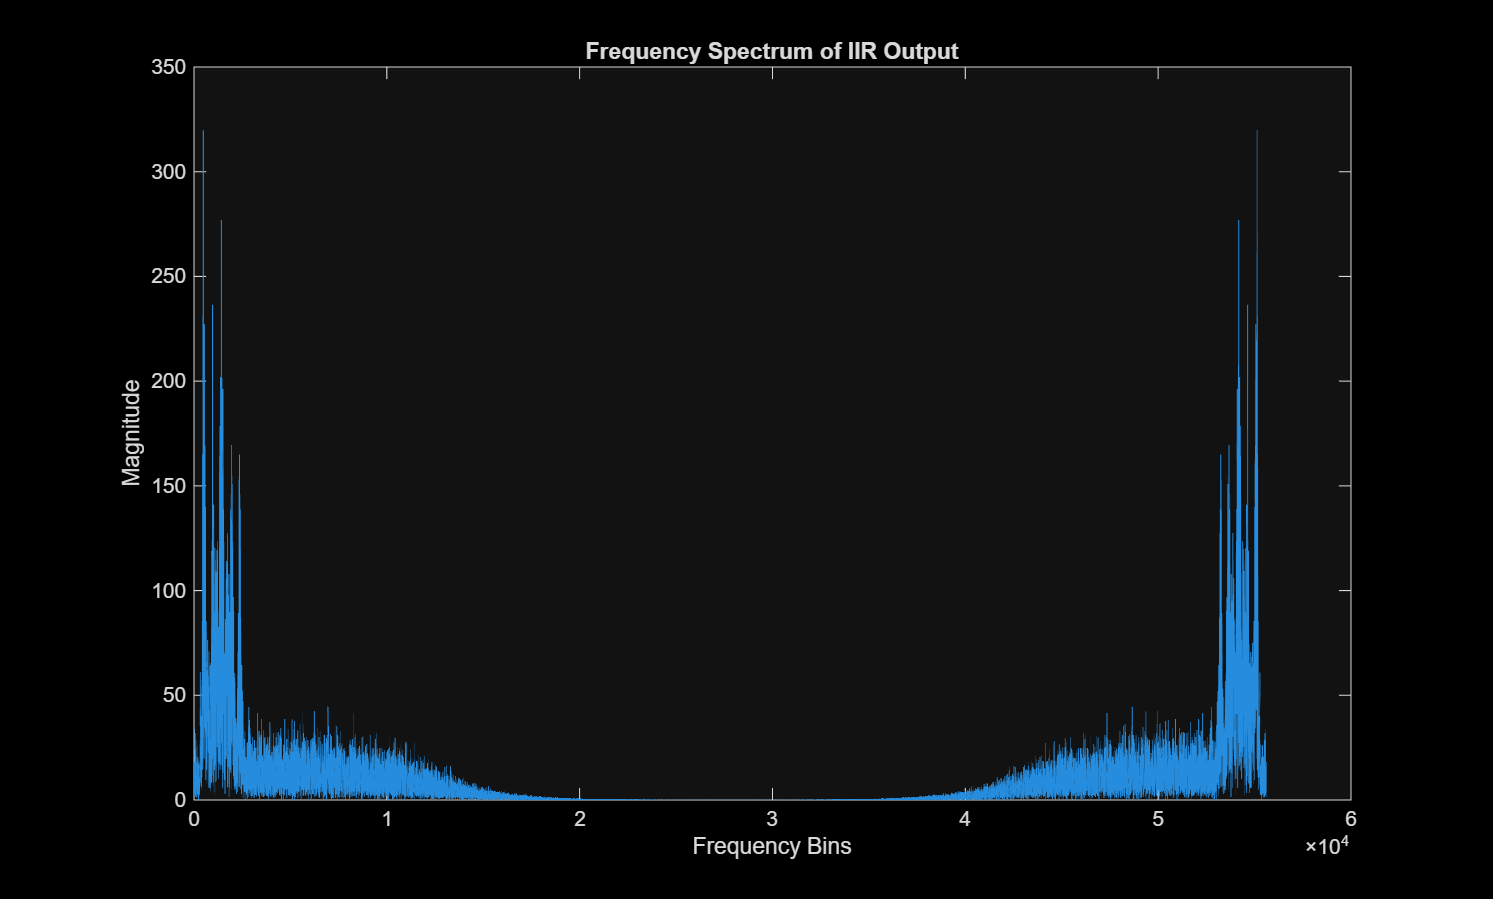
\includegraphics[width=0.48\columnwidth,height=3.3cm,keepaspectratio]{fft_iir.png}
}
\caption{Frequency-domain comparison of the original, noisy, and filtered speech signals}
\label{fig:fft_group}
\end{figure}

After applying the FIR and IIR filters, a reduction in high-frequency components can be observed. This indicates that the filters are able to suppress noise to some extent.

The frequency responses of the filters further explain their behavior. Both filters act as low-pass filters, allowing lower frequency components of speech to pass while attenuating higher frequency noise.

\begin{figure}[htbp]
\centering
\subfloat[Frequency response of FIR filter]{
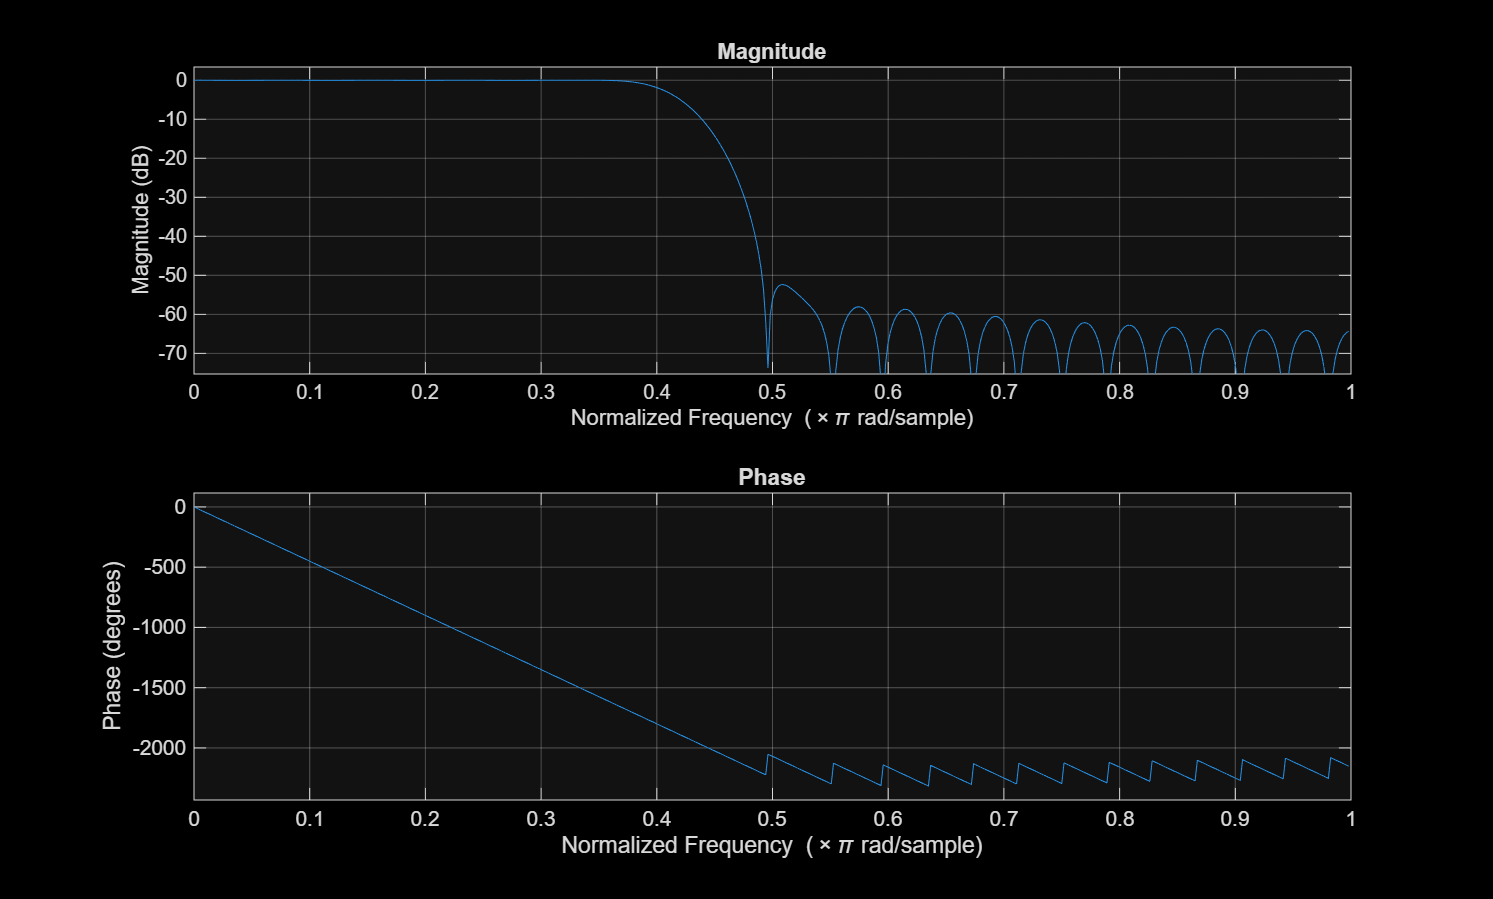
\includegraphics[width=0.48\columnwidth,height=3.3cm,keepaspectratio]{fir_response.png}
}
\hfill
\subfloat[Frequency response of IIR filter]{
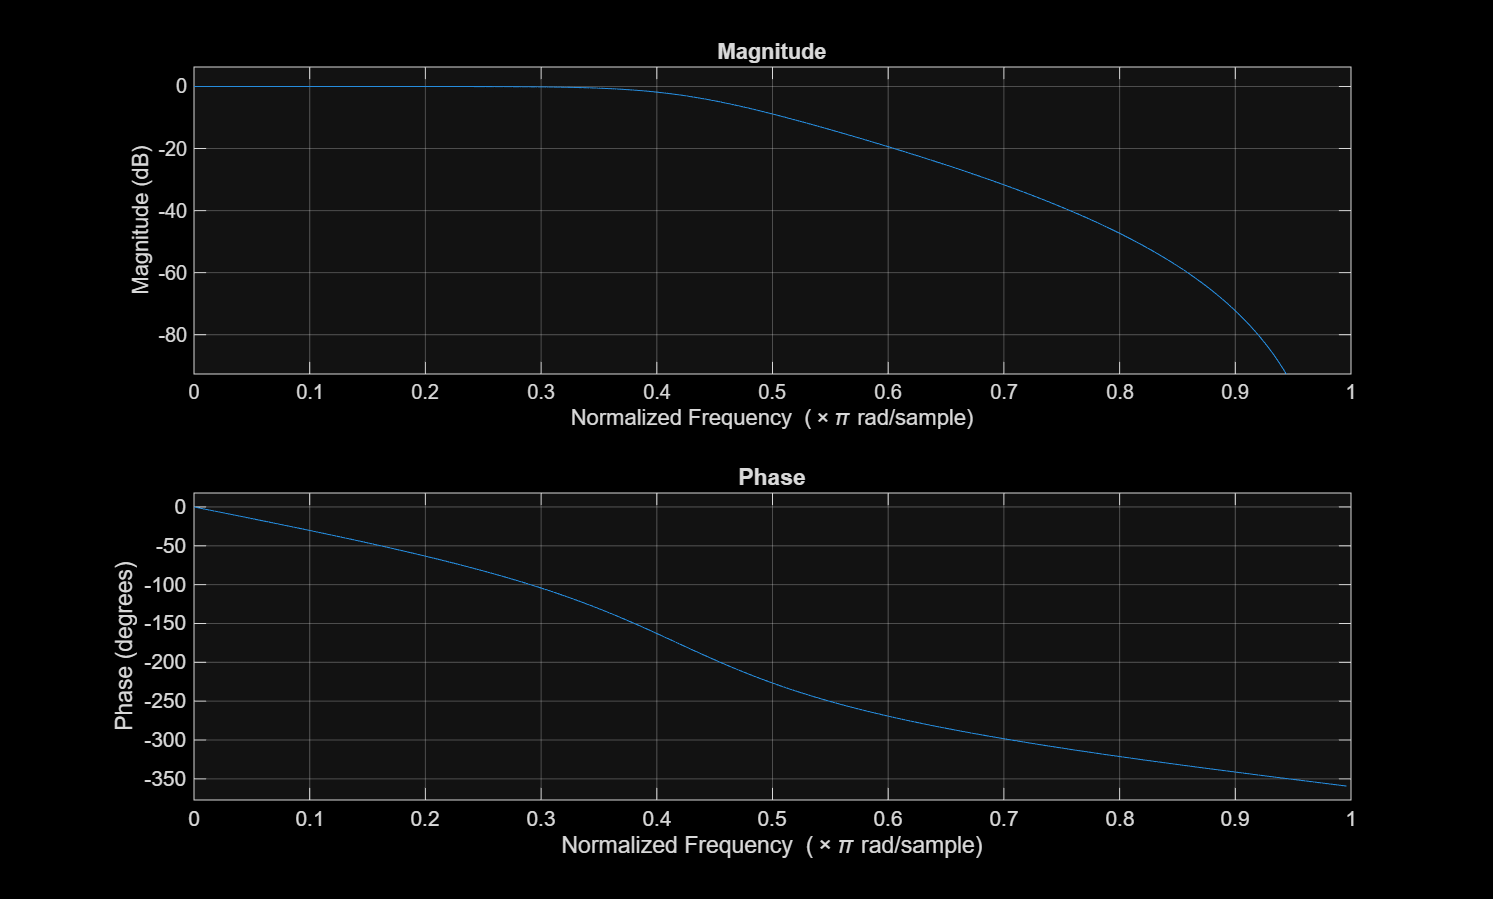
\includegraphics[width=0.48\columnwidth,height=3.3cm,keepaspectratio]{iir_response.png}
}
\caption{Frequency responses of the FIR and IIR filters}
\label{fig:filter_response_group}
\end{figure}

From the frequency-domain analysis, it is evident that the IIR filter provides a sharper transition in frequency response, which helps in better noise suppression. The FIR filter, although smoother, shows less effective attenuation in this case, which is consistent with the quantitative results obtained earlier.

\subsection{Subjective Evaluation}

In addition to visual and quantitative analysis, the quality of the processed speech signals was also evaluated through listening.

The noisy signal was found to contain noticeable background noise, which reduced the clarity of the speech. After applying the FIR filter, the signal appeared smoother, but some distortion in the speech components was observed.

The IIR filter provided a clearer output with better preservation of speech characteristics. The background noise was reduced more effectively, and the speech was more intelligible compared to the FIR output.

These observations are consistent with the quantitative results, where the IIR filter showed improvement in SNR and lower MSE. This indicates that the IIR filter performs better for the given speech enhancement task.

\section{Summary of Results}

A comparison between the FIR and IIR filters is presented in Table~\ref{tab:comparison}. The comparison highlights the key characteristics observed during the implementation and analysis.

\begin{table}[htbp]
\caption{Comparison between FIR and IIR filters}
\centering
\begin{tabular}{|c|c|c|}
\hline
\textbf{Parameter} & \textbf{FIR Filter} & \textbf{IIR Filter} \\
\hline
Structure & Non-recursive & Recursive \\
\hline
Stability & Always stable & Conditionally stable \\
\hline
Phase Response & Linear phase & Non-linear phase \\
\hline
Computation & More computations & Less computations \\
\hline
Efficiency & Lower & Higher \\
\hline
Output Quality & Smooth signal & Clear signal with fast response \\
\hline
\end{tabular}
\label{tab:comparison}
\end{table}

From the comparison, it can be observed that FIR filters provide a stable and smooth output due to their linear phase characteristics. However, they require higher computational effort and may not always achieve sharp filtering with lower orders.

On the other hand, IIR filters are more efficient and require fewer coefficients to achieve a sharper frequency response. This results in better noise suppression with lower computational cost.

The observations from this comparison are consistent with the results obtained in the previous sections. The IIR filter shows an improvement in SNR and a reduction in MSE, indicating better performance in noise reduction. In contrast, the FIR filter shows degraded performance in this case, which can be attributed to non-optimal filter design parameters such as cutoff frequency and filter order.

This analysis highlights that while FIR filters are theoretically stable and reliable, IIR filters can provide better practical performance when properly designed.

\section{Conclusion}

In this work, a simple speech enhancement system using digital signal processing techniques has been presented. The system focuses on reducing noise from a speech signal using FIR and IIR filters. A clean speech signal was taken, noise was added, and both filters were applied to improve the signal quality.

The results show that both FIR and IIR filters are effective in reducing noise. The FIR filter provides a stable output and maintains the shape of the signal, while the IIR filter achieves similar results with lower computational effort. This makes the IIR filter more efficient for practical applications.

The implementation in MATLAB helps in understanding the basic concepts of digital filtering and speech enhancement in a clear and practical manner. Overall, the work demonstrates that simple filtering techniques can be used to improve speech quality without using complex methods.

\section{Limitations}

Although the proposed speech enhancement system demonstrates the basic effectiveness of FIR and IIR filters, it has certain limitations.

The current implementation considers only additive white Gaussian noise. In real-world scenarios, speech signals may be affected by different types of noise such as background conversations, environmental sounds, or non-stationary noise, which are more challenging to remove.

The filter parameters used in this work, such as cutoff frequency and filter order, are fixed and not optimized for different conditions. As observed in the results, this can lead to suboptimal performance, particularly in the case of the FIR filter.

The system is implemented in an offline manner and does not support real-time processing. Additionally, adaptive filtering techniques are not considered, which could improve performance in dynamic environments.

These limitations indicate that while the current approach is suitable for basic understanding and demonstration, further improvements are required for practical applications.

\section{Future Work}

The current work focuses on basic speech enhancement using FIR and IIR filters under simple noise conditions. Based on the limitations identified, several improvements can be considered in future.

One possible extension is the use of adaptive filtering techniques such as Least Mean Squares (LMS) and Normalized LMS (NLMS), which can adjust filter parameters dynamically and perform better in changing noise environments.

More advanced methods such as spectral subtraction and Wiener filtering can also be explored to achieve improved noise reduction performance.

In addition, machine learning and deep learning-based approaches can be used for speech enhancement, especially in complex and non-stationary noise conditions.

Another important improvement is the implementation of the system for real-time processing, which would make it suitable for practical applications such as communication systems and assistive devices.

Further work can also include optimizing filter parameters for different types of noise and testing the system with a wider range of speech signals.

\begin{thebibliography}{00}

\bibitem{b1} A. V. Oppenheim and R. W. Schafer, \textit{Discrete-Time Signal Processing}, 3rd ed. Upper Saddle River, NJ, USA: Prentice Hall, 2010.

\bibitem{b2} J. G. Proakis and D. G. Manolakis, \textit{Digital Signal Processing: Principles, Algorithms, and Applications}, 4th ed. Upper Saddle River, NJ, USA: Pearson, 2007.

\bibitem{b3} MathWorks, ``Audio Processing in MATLAB,'' Available: https://www.mathworks.com/help/audio/

\bibitem{b4} S. Boll, ``Suppression of acoustic noise in speech using spectral subtraction,'' IEEE Trans. Acoustics, Speech, and Signal Processing, vol. 27, no. 2, pp. 113--120, Apr. 1979.

\bibitem{b5} B. Widrow and S. D. Stearns, \textit{Adaptive Signal Processing}. Englewood Cliffs, NJ, USA: Prentice Hall, 1985.

\bibitem{ref6}
Y. Ephraim and D. Malah, “Speech enhancement using a minimum mean-square error short-time spectral amplitude estimator,” IEEE Transactions on Acoustics, Speech, and Signal Processing, vol. 32, no. 6, pp. 1109–1121, Dec. 1984.

\bibitem{ref7}
P. C. Loizou, \textit{Speech Enhancement: Theory and Practice}. Boca Raton, FL, USA: CRC Press, 2013.

\bibitem{ref8}
S. F. Boll, “Suppression of acoustic noise in speech using spectral subtraction,” IEEE Transactions on Acoustics, Speech, and Signal Processing, vol. 27, no. 2, pp. 113–120, Apr. 1979.

\end{thebibliography}

\end{document}
